% Preamble
\documentclass[11pt]{article}
% Packages
\usepackage{ngerman}
\usepackage{amsmath}
\usepackage{url}
\usepackage{graphicx}
\usepackage{float}
\usepackage{pifont}

\title{\textbf{Konzepte} zur Bachelorarbeit\\\large{Template-basierte Synthese von\\Verzweigungsstrukturen mittels
L-Systemen}}
\author{Adrian Helberg}

% Document
\begin{document}
    \maketitle
    \tableofcontents
    \newpage
    \section{Softwareprojekt}
    \subsection{Vorgehensmodell}
    Eine Fallstudie der Universität Karlsruhe\cite{1} untersucht den Einsatz der Softwaretechnik \textbf{Extreme Programming}
    (XP) im Kontext der Erstellung von Abschlussarbeiten im Universitätsumfeld.\\~\\
    Hierzu werden folgende Schlüsselpraktiken untersucht:
    \begin{itemize}
        \item XP als Softwaretechnik zur schrittweisen Annäherung an die Anforderungen eines Systems
        \item Änderung der Anforderungen an das Systems
        \item Funktionalitäten (\textbf{Features}) werden als Tätigkeiten des Benutzers (\textbf{User Stories}) definiert
        \item Zuerst werden Komponententests (Modultests) geschrieben und anschließend die Features (Test-driven Design)
        \item Keine seperaten Testing-Phasen
        \item Keine formalen Reviews oder Inspektionen
        \item Regelmäßige Integration von Änderungen
        \item Gemeinsame Implementierung (Pair Programming) in Zweiergruppen
    \end{itemize}
    Aus der Fallstudie geht hervor, dass Extreme Programming einige Vorteile bei der Bearbeitung eines Softwareprojektes
    einer Bachelorarbeit bietet.
    Zum einen können sich Anforderungen an das zu erstellende System durch parallele Literaturrecherche ändern, zum
    anderen können die Arbeitspakete durch Iterationen abgedeckt werden.
    \newpage

    \subsection{Vorgehen}
    Das Programm zu dieser Arbeit wird mit einem XP-basierten Ansatz erarbeitet.
    Hierbei beinhaltet ein \textbf{Release} Funktionen, die insgesamt für eine neue Version des Systems ausreichen;
    also ein vollständig funktionsfähiges Programm liefern.
    \textbf{User Stories} sind innerhalb der Iterationen umzusetzende Teilaufgaben und deren Aufwandseinschätzung gibt
    Auskunft über den Entwicklungsaufwand einer Umsetzung.\\~\\
    Umsetzung des Softwareprojektes in Iterationen mit folgenden Phasen:
    \begin{itemize}
        \item Planung:
        \begin{itemize}
            \item Release-Planung:\\"`\textit{Welche Features werden in diesem Release umgesetzt?}"',\\User Stories,
            Aufwandsschätzung, Anforderungsmanagement
            \item Iterationsplanung:\\Umwandlung der User Stories in kleine Arbeitsschritte,\\Festlegen der Dauer einer
            Implementierung
        \end{itemize}
        \item Entwurf: Architektur, Klassendiagramme
        \item Testing: (Automatisierte) Modultests und Regressionstests
        \item Programmierung: Umsetzung der Features, Implementierung
    \end{itemize}
    \begin{figure}[H]
        \centering
        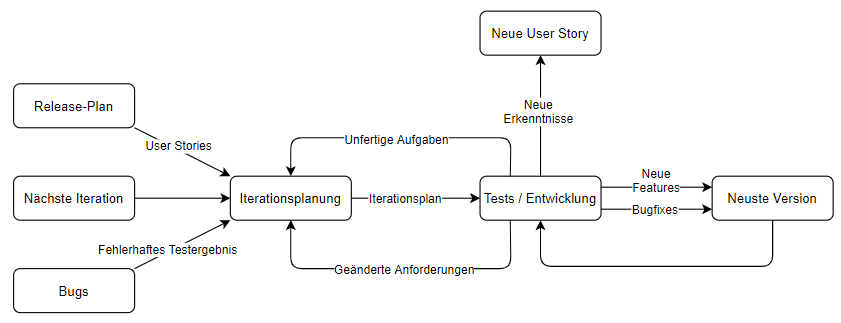
\includegraphics[width=15cm]{../images/extreme_programming.PNG}
        \caption{Ablaufdiagramm}
    \end{figure}

    \subsection{Technnologien}
    \begin{itemize}
        \item Programmiersprache: Java Version X
        \item Versionskontrolle: Github Repo
        \item IDE: JetBrains IntelliJ IDEA 2020.2.2 (Ultimate Edition)
        \item Betriebssystem: Microsoft\textregistered Windows 10 Pro 64 Bit
        \item Prozessor: Intel\textregistered Core\texttrademark i5-3570K CPU @ 3.40GHz
    \end{itemize}

    \newpage

    \section{Dokumentation}
    \subsection{Gliederung}
    Im Folgenden wird eine vorläufige Gliederung der schriftlichen Ausarbeitung gezeigt
    \begin{itemize}
        \item[1.] Abbildungs- und Tabellenverzeichnis
        \item[2.] Abkürzungsverzeichnis
        \item[3.] Einleitung
        \begin{itemize}
            \item[3.1.] Problemstellung
            \item[3.2.] Ziele
            \item[3.3.] Methodik
            \item[3.4.] Aufbau
        \end{itemize}
        \item[4.] Grundlagen
        \begin{itemize}
            \item[4.1.] Grundbegriffe
            \item[4.2.] Grundlegende Arbeiten
            \item[4.3.] Verwandte Arbeiten
        \end{itemize}
        \item[5.] Konzepte
        \begin{itemize}
            \item[5.1.] Probleme \& Lösungsansätze
            \item[5.2.] Architektur
            \item[5.3.] Algorithmen
        \end{itemize}
        \item[6.] Implementierung
        \item[7.] Evaluierung
        \begin{itemize}
            \item[7.1.] Testumgebung
            \item[7.2.] Beobachtungen \& Ergebnisse
            \item[7.3.] Diskussion und Bewertung
        \end{itemize}
        \item[8.] Ausblick
        \item[9.] Literaturverzeichnis
        \item[10.] Eidesstattliche Erklärung
    \end{itemize}

    \section{Quellen}

    ~\nocite{*}
    \bibliography{konzepte}
    \bibliographystyle{plain}

\end{document}